\documentclass[12pt]{article}
%%%%%%%%%%%%%%%%%% General pagackages
\usepackage{amssymb,amsmath,amsfonts,eurosym,ulem,graphicx,
	caption,color,setspace,sectsty,comment,footmisc,
	pdflscape,subcaption,array, multicol,multirow,tikz, bm,
        booktabs, rotating, titling}     
%%%%%%%%%%%%%%%%%%% Encoding
\usepackage[utf8]{inputenc}
%%%%%%%%%%%%%%%%%% Margins and Spacing
\usepackage[left=1.0in,right=1.0in,top=1in,bottom=1in]{geometry}
\usepackage{indentfirst}
%%%%%%%%%%%%%%%%%% References
\usepackage[sort]{natbib}
\bibliographystyle{econ}
%%%%%%%%%%%%%%%%%% Links
\usepackage[colorlinks=true, allcolors=blue]{hyperref}
\urlstyle{same} %makes url the same font as text, not courier default
\newcommand{\doi}[1]{\url{#1}}
%%%%%%%%%%%%%%%%%% tikz/diagrams
\usetikzlibrary{arrows,shapes,positioning,intersections,calc}
%%%%%%%%%%%%%%%%%% table formatting
\newcolumntype{L}[1]{>{\raggedright\arraybackslash}p{#1}}
\newcolumntype{C}[1]{>{\centering\arraybackslash}p{#1}}
\newcolumntype{R}[1]{>{\raggedleft\arraybackslash}p{#1}}
\normalem
\makeatother
%%%%%%%%%%%%%%%%%% Autoreference names
\renewcommand{\sectionautorefname}{Section}
\renewcommand{\subsectionautorefname}{Sub-section}
\renewcommand{\figureautorefname}{Figure}
\renewcommand{\tableautorefname}{Table}
\renewcommand{\figureautorefname}{Figure}
% equation numbering start at 1
\newcommand\numberthis{\addtocounter{equation}{1}\tag{\theequation}}
%%%%%%%%%%%%%%%%%% Theorem Names
\newtheorem{prop}{Proposition}
\newtheorem{definition}{Definition}
\newtheorem{lemma}{Lemma}
\newtheorem{corollary}{Corollary}
\newtheorem{result}{Result}
\newtheorem{assumption}{Assumption}
\newtheorem{theorem}{Theorem}

%%%%%%%%%%%%%%%%%% Title Information
%title page single spacing 
\setstretch{1} 
%subtitle command
\newcommand{\subtitle}[1]{\posttitle{\par\end{center}\begin{center}\large#1\end{center}\vskip0.5em}}

\title{All Tables and Charts}
\subtitle{Brown University\\Honors Thesis in Economics}

\begin{document}

\maketitle


\begin{figure}[ht]
    \centering
    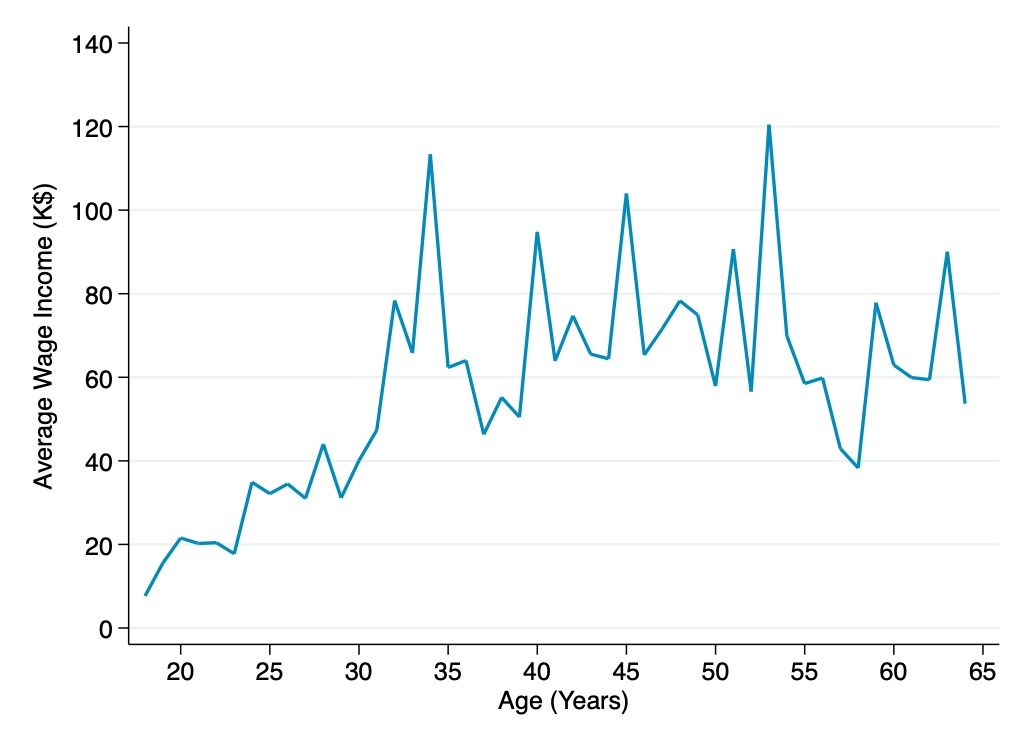
\includegraphics[width=.75\textwidth]{figures/avgwageincome_wage.jpg}
\end{figure}



\begin{table}[ht]
    \centering
    \caption{Summary Statistics}
    {
\def\sym#1{\ifmmode^{#1}\else\(^{#1}\)\fi}
\begin{tabular}{l*{1}{ccccc}}
\toprule
                    &        Mean&          SD&         Min&         Max&           N\\
\midrule
Wage income         &      58.734&      71.836&           1&         850&         835\\
Total income        &   63924.501&   79303.953&        1000&      957500&         835\\
Age                 &      40.941&      12.462&          18&          64&         835\\
Female              &       0.497&       0.500&           0&           1&         835\\
White               &       0.734&       0.442&           0&           1&         835\\
Black               &       0.143&       0.350&           0&           1&         835\\
Married             &       0.571&       0.495&           0&           1&         835\\
In labor force      &       1.000&       0.000&           1&           1&         835\\
\bottomrule
\end{tabular}
}

\end{table}



\begin{table}[ht]
    \centering
    \caption{Regression Results}
     {
\def\sym#1{\ifmmode^{#1}\else\(^{#1}\)\fi}
\begin{tabular}{l*{4}{c}}
\toprule
                    &\multicolumn{1}{c}{(1)}&\multicolumn{1}{c}{(2)}&\multicolumn{1}{c}{(3)}&\multicolumn{1}{c}{(4)}\\
                    &\multicolumn{1}{c}{Total income}&\multicolumn{1}{c}{Total income}&\multicolumn{1}{c}{Total income}&\multicolumn{1}{c}{Total income}\\
\midrule
Female              &    -22883.7\sym{***}&    -20939.8\sym{***}&    -21827.8\sym{***}&    -18064.1\sym{***}\\
                    &    (4729.3)         &    (4323.2)         &    (4324.8)         &    (4481.8)         \\
\addlinespace
Constant            &     75297.8\sym{***}&     74331.7\sym{***}&     74697.4\sym{***}&     72243.4\sym{***}\\
                    &    (2350.5)         &    (2148.7)         &    (2149.4)         &    (2249.4)         \\
\midrule
Observations        &         835         &         835         &         833         &         787         \\
\(R^{2}\)           &       0.084         &       0.188         &       0.201         &       0.340         \\
State FE            &         Yes         &         Yes         &         Yes         &         Yes         \\
Age FE              &          No         &         Yes         &         Yes         &         Yes         \\
Race FE             &          No         &          No         &         Yes         &         Yes         \\
Industry FE         &          No         &          No         &          No         &         Yes         \\
\bottomrule
\end{tabular}
}

\end{table}

\end{document}
